% This is samplepaper.tex, a sample chapter demonstrating the
% LLNCS macro package for Springer Computer Science proceedings;
% Version 2.20 of 2017/10/04
%
\documentclass[runningheads]{llncs}
%
\usepackage{mwe}
\usepackage{graphicx}
\graphicspath{{figures/}}
\usepackage{color}
\definecolor{highlight}{rgb}{1,1,0.6}
\definecolor{link}{rgb}{0.5,0.0,0.0}
\definecolor{cite}{rgb}{0.0,0.0,0.6}
\definecolor{url} {rgb}{0.3,0.0,0.3}
\definecolor{grey}{rgb}{0.3,0.3,0.3}

\usepackage[hidelinks]{hyperref}
\hypersetup{
	colorlinks,
	linkcolor={cite},
	citecolor={cite},
	urlcolor ={cite}
}

\usepackage{tabularx}
\usepackage{array}
\usepackage{booktabs} % for nice rules/lines in tables
\usepackage{arydshln} % for dashed lines in tables

\usepackage{soul} % for highlighting text
\usepackage{xspace}
\usepackage[shortcuts]{extdash}
\usepackage{relsize} % used in the \anote and \comment macros.

%% annotation commands %% 
\newcommand{\anote}[1]{{\leavevmode\smaller\itshape\color{red}\{#1\}}}
\sethlcolor{highlight}
\newcommand{\comment}[2]{\hl{#1} {{\leavevmode\smaller\color{red}\itshape\{#2\}}}}

%% PM Define authornote command for comments
\newcommand{\authornote}[1] {
	\begin{center}
		\framebox{
			{\begin{minipage}[t]{0.9\linewidth}
					\raggedright  \textbf{[PM]}~ \scriptsize #1 \normalsize
			\end{minipage}}
		}
	\end{center}
}

\newcommand*{\bibfont}{\tiny}



\newcommand{\demon}{{DEMON}}
\newcommand{\infomap}{{Infomap}}

\usepackage{amssymb}
\usepackage{bm}
\usepackage{mathtools}

% custom commands
\usepackage{rotating}
\newcolumntype{P}[1]{>{\centering\arraybackslash}p{#1}}
\newcolumntype{Y}{>{\centering\arraybackslash}X}
\usepackage{subcaption}


\begin{document}
%
\title{Fantastic activists and how to find them\thanks{}}
%
%\titlerunning{Abbreviated paper title}
% If the paper title is too long for the running head, you can set
% an abbreviated paper title here
%
\author{First Author\inst{1}\orcidID{0000-1111-2222-3333} \and
Second Author\inst{2,3}\orcidID{1111-2222-3333-4444} \and
Third Author\inst{3}\orcidID{2222--3333-4444-5555}}
%
\authorrunning{F. Author et al.}
% First names are abbreviated in the running head.
% If there are more than two authors, 'et al.' is used.
%
\institute{affiliation 1 \and
Springer Heidelberg, Tiergartenstr. 17, 69121 Heidelberg, Germany
\email{lncs@springer.com}\\
\url{http://www.springer.com/gp/computer-science/lncs} \and
ABC Institute, Rupert-Karls-University Heidelberg, Heidelberg, Germany\\
\email{\{abc,lncs\}@uni-heidelberg.de}}
%
\maketitle              % typeset the header of the contribution
%
\begin{abstract}
last to be written
\keywords{Twitter analytics  \and online user discovery \and online activists \and influencers}
\end{abstract}
%


%
%
\section{Introduction}

In this paper we present a generic and customisable software  framework for incrementally discovering and ranking online individuals' profiles for classes of online users, through analysis of their social activity in micro-blogging platforms, specifically Twitter.
While the framework can be customised to repeatedly search for and rank profiles that fit specific social roles, our work is motivated by the specific need to discover a special class of such users, which we call \textit{activists}. 
We start by arguing for the need for a new discovery process for this class of users, and then we present the framework as our main research contribution.

According to the Cambridge Dictionary, an \textit{activist} is  ``A person who believes strongly in political or social change and takes part in activities such as public protests to try to make this happen''.

While activism is well-documented, e.g. in the social movement literature~\cite{doi:10.1080/14742830701497277}, and online activism is a well-known phenomenon \cite{IJoC1246}, research has been limited to the study of its broad societal impact. 
In contrast, we are interested in the fine-grained discovery of activists at the level of the single individual, in other words, we seek to identify people who feel passionate about a cause or topic, and who take action for it. 
Searching for online activists is a realistic goal, as activists presence in social media is widely acknowledged, and it is also clear that social media facilitates activists communication and organization \cite{Poell2014,Youmans2012}.  
Specific traits that characterise activists include awareness of causes and social topic and the organization of social gatherings and activities, including in emergency situations, by helping organize support efforts and diffusion of useful information.
 
Informal as it sounds, this characterisation of online activism is different from that of \textit{influencer}.
According to ~\cite{Kardara2015}, \textit{influencers are prominent individuals with special characteristics that enable them to	affect a disproportionately large number of their peers with their actions.}
A large number of metrics and techniques have been proposed over an extended period of research, to make this generic definition operational~\cite{RIQUELME2016949}. These are mostly based on metrics of network centrality, along with metrics derived from the users' online activity, i.e., number of retweets or other users' content, number of retweets of own content, and many more.

Algorithms to find influencers favour high visibility profiles, typically across global networks.
In contrast, activists are more low-key, less prominent users who only emerge from the crowd by signalling high levels of engagement with one or more specific topics, as opposed to being thought-leaders.
%
While we believe that specific activist behaviour can be characterised using some of the well-tested quantifiable metrics known from the literature \cite{COMMON-METRICS}, it should also be clear that the way such metrics are combined to identify activist profiles are not the same as for influencers. 

Motivated by these observations, our search for activists faces two main problems.
%
Firstly, we note that, given the more subdue nature of activists, it is intuitively more difficult to separate their online footprint from the background noise of general conversations, than it is for an influencer.
Also, interesting activists are by their nature associated to specific topics and manifest their nature in local contexts, for instance as organisers or participants to local events. 
Finally, we seek evidence of sustained personal engagement over time and across multiple such contexts. 
These observations suggest that the models and algorithms developed over the years for influencers are not immediately applicable, because they mostly operate on global networks, where less prominent users have less of a chance to emerge. 
Some topic-sensitive metrics and models have been proposed to measure social influence, for example, \textit{alpha centrality}\cite{Bonacich2001,Overbey2013}, and the \textit{Information Diffusion} model. Algorithms based on topic models have also been proposed to account for topic specificity~\cite{Zhao2011b}.  However, these approaches are still aimed at measuring influence, not activism. 

Secondly, our definition of activism requires proper formalisation, i.e., in terms of measurable metrics, as well as experimental validation. 

The approach we propose to address these problems involves two strategies. 
Firstly, we first identify suitable contexts that are topic-specific and bound both temporally and, optionally, also spatially.
We then search for users only within these contexts, using a combination of network and content metrics. 
Given the nature of our target users, these include a combination of social events and online campaigns, as illustrated later \textbf{REF}.
This follows the intuition that low-key users who produce weak online signal have a better chance to be discovered when the search is localised and then repeated across multiple such contexts.
By continuously finding new contexts and searching for users engaged in the events and campaigns, we hope to incrementally build up a users' database where users who appear in multiple events are progressively more strongly characterised.

Secondly, to allow experimenting with varying technical definitions of \textit{activist}, we collect a number of network-based and content-based user profile metrics, and make it available into a database. 

we have developed a generic but customisable processing pipeline for Twitter, 



\authornote{OLD TEXT BELOW}











	


\anote{A broader motivation for the approach we present here is that relatively low-profile users are hard to identify by using traditional approaches based on global content harvesting and large Twitter networks.}

\anote{what the work is really about:
	
	a configurable framework to incrementally generate datasets of Twitter users, along with a rich set of features,  pre-selected from limited contexts to be a more varied set than global influencers
	 
	the resulting database can be mined to extract a variety of user types, by combining
	
	we demonstrate

}

\anote{a critique of established network methods to identify these particular profiles:
\begin{itemize}
%	\item activists are users who are interesting but not in the same sense as influencers (many defs). but these are ``low-key'' users who are not famous or at the centre of large networks. 
	\item Thus discovering such users is hard because they ``disappear in the noise'' of a large global social network with a very broad range of topics.
%	\item traditional approaches don't work well for these profiles. (this is a bit axiomatic - not proven)
\end{itemize}
}



In contrast, in our current incremental approach, the idea is to first discover one or more online contexts associated with a topic, such as a social campaign or a local event.
Our hypothesis is that each such  context provides a low-noise scope within which those users who would not otherwise be identified using standard network analysis techniques, are given a chance to ``stand out'' and emerge, as the limited scope may amplify their otherwise weak signal and isolate them from some of the global participants.

We also make the hypothesis that, within each such focused context, we maybe able to  successfully use established social network metrics to identify users who are active within the context, i.e., those who engage in meaningful interactions that provide a limited but strong signal about their interest in the chosen topic. 
%
As contexts are temporally (and optionally also spatially) characterised, this approach also lends itself well to incremental user discovery,  and to building strong profiles of users who are observed in multiple contexts over time.


\anote{Zika angle probably too specific so the below is parked:
\begin{itemize}

\item Mosquito-borne diseases such as Zika, Dengue and Chikungunya are endemic in several countries and Brazil is one of the most affected ones.
\item These diseases cause severe symptomatic effects and complications which include hemorrhagic fever and microcephaly in newborns of contaminated mothers.
\item Why they are difficult to fight: No vaccines available, Government is ineffective, slow and has low resources
\end{itemize}

Our long-term goal is to help alleviate these problems by supporting the health officials in their efforts to detect and clean up mosquito breeding sites.
Thus, in a practical sense our study is on techniques for identifying those individuals who are likely to become engaged with volunteering efforts.
Note that we are not seeking people who have shown  specific interest in the fight against Zika or other epidemics, but rather, more generally, we are looking for people who have a recent and sustained history of social engagement. 
%
}


\anote{moved from techapproach}

As mentioned in the introduction, the main limitation of our own previous approach 	\cite{Missier2017,Sousa2018,Barros2018} is that topology-based metrics such as h-index and centrality analysis could not be used, because the users identified through the content relevance approach led to collections of disconnected users. Essentially, each user would be considered relevant in isolation, but on the basis of a very sparse signal.
%
At the same time, traditional approaches aimed at discovering influential users, surveyed for instance in \cite{RIQUELME2016949}, require large and connecTwitterRank and rely on large social networks do not work well when the users we are seeking a 


\anote{this may not be needed?  depending on space}

\anote{
	the definition of activists is based on a few established metrics. we do not invent new metrics but we combine a few that exist in a way that is justified intuitively, by drawing from literature on online activism.
	
	the metrics include (1) content-based, non-topological metrics based on a user's post history
	
	(2) non-contextual topological
	
	(3) non-contextual topological.
	
	in past approaches, specific profiles, such as those of influencers and many others \cite{RIQUELME2016949}, have been proposed. these essentially combine a set of basic metrics.
	
	call these \textit{engineered features}. 
}


\anote{Candidate discovery is based on a weak notion of online event. It is \textit{weak} because on Twitter events are not explicitly defined, unlike for example in Facebook or Meetup.}

\anote{Our technique achieves two things:
	
	\begin{itemize}
		\item discover candidate Twitter profiles
		\item repeatedly measure the \textit{strength} of candidate profiles as activists over time, thus enabling dynamic profile ranking
	\end{itemize}	
}

\anote{clarify that when we say ``social media'' in this paper we refer exclusively to Twitter. So I guess just as well say Twitter explicitly everywhere? }



\anote{
	The main insight behind the process structure is to first identify suitable contexts (online campaigns, events around social issues) where the target user profiles stand out relative to the global network. 
	
	Rationale: observing users in context has the effect of drastically reducing the noise of general Twitter signal, relative to the general stream.  
	
	
	Context discovery is currently the only step where human intervention is required (but that can be crowd-sourced as it does not involve deep specialist knowledge).
	
	\begin{itemize}
		\item Conversations that take place within the context of an event are represented as dynamic weighted social network graphs (context network)
		
		\item Depending on the size and importance of the event, these networks may be first partitioned into smaller virtual overlapping communities, using the Demon community detection algorithm. \textbf{Rationale} for this: users who are low profile within the larger graph may emerge within a more local community. This is the same rationale as for the general ideas of  contexts)
		\item users within each community (for small communities, we use the entire network) are then ranked according to some combination of all their features
		\item Progressively build up stronger profiles of repeat users, by updating their strength using the new values for the metrics
	\end{itemize}
}

\comment{Since our method relies on small networks that represent limited topical context, our challenge is to find metrics that operate well on small networks.}{rephrase}



\subsection{Reference case study and running example}  \label{sec:reference}

\anote{where we are looking for activists. This case study is intended to meet our original motivation, while demonstrating the user discovery process in action. There is no separate ground truth validation so this intends to show how the framework works when you choose topics for the contexts, and a specific set of metrics.}

\subsection{Paper contributions}

The paper offers the following specific contributions.
\begin{itemize}
\item We propose a semi-automated, incremental process for identifying \textit{low-profile} users who are characterised by a weak online signal, i.e., they are not ``global influencers'', and yet they are interesting as they show interest in actively engaging with social issues online. 

\item As a concrete example of the process in use, we characterise our target users as ``online activists '' by proposing an operational definition of their profiles in terms of well-established, quantifiable Twitter metrics which can be used;

\item A reference implementation of the process and its demonstration on a reference case for online activism in the \hl{XX} domain;

\item A performance evaluation to assess the impact of the Twitter API limitations on content retrieval, specifically sampling from the ``garden hose'' 
\anote{FLAVIO: from my understanding garden hose twitter api is a daily streaming API which we don't use http://www.sobigdata.eu/content/twitter-stream-gardenhose-daily-access }
\end{itemize}

\subsection{Related Work}


\anote{topic-specific influencers. cite \cite{Schenk2011} SCHENK 2011 and 
	
	\cite{Kardara2015} KARDARA:
	Here a new ranking algorithm is proposed to find local influencers on Twitter that appear within the context of a specific event being discussed, incorporating the network dynamics as the event evolves with time. 
	Local to an event conrtext but focus on user reputation. 
	The above techniques all attempt to define influence as
	some measurable attribute or observation in the network, such as how many times an original story appears on a website, or how centrally connected a node is within various defined modules within the networks.
	The definition used in this work for influ-ence is “who is being listened to the most”.
	- this is not who we are looking for.
	- one single large event
	- no breakdown into communities
}


%%%%%%%%%%%%%%%%%%%%%
\section{Incremental User discovery}
%%%%%%%%%%%%%%%%%%%%%

\subsection{Contexts} \label{sec:contexts}

As described In Sec. ~\ref{sec:reference}, contexts are meant to identify events or campaigns around social issues, which are characterised by temporal boundaries and by hashtags and/or keyword terms, and optionally also by spatial constraints, i.e., specified using a geographical bounding box.
In the Twitter settings we refer to these as \textit{weak} contexts, because Twitter does not natively support the notion of event or campaign (unlike, for example, Facebook, Instagram, or Meetup).
We  denote a generic context as
\begin{equation}
C = \langle s, [t_1, t_2], K \rangle 
\label{eq:context}
\end{equation}
where  $s$ represents the optional spatial constraint, $[t_1, t_2]$ a time interval, and $K = \{ k_1 \dots k_n\}$ is the set of terms used to filter content within the spatio-temporal boundaries.
%
$C$ defines search criteria, which produce a set $T(C)$ of tweets when submitted to Twitter.
We only consider two Twitter activities: an \textit{original tweet}, or a \textit{retweet}.
Let $u(t)$ be the user who originated a tweet $t \in T$.
We say that both $t$ and  $u(t)$ are \textit{within context} $C$.

We also define the complement $\Tilde{T}(C)$ of $T(C)$ as the set of tweets found using the same spatio-temporal constraints, but which do not contain any of the terms in $K$. More precisely, given a  context $C'= \langle s, [t_1, t_2], \emptyset \rangle$, we define $\Tilde{T}(C) = T(C') \setminus T(C)$. 
We refer to these tweets, and their respective users, as ``out of context $C$''.



\subsection{Features  for online activists}

For the purpose of our case study, we adopt a specific small set of such metrics, which together form   the basis for an operational definition of \textit{online activist}.
The choice of metrics follows broadly the indications found in recent studies on online activism, namely \cite{Lotan2011} and  \cite{Poell2014}, and is as follows.

For \textbf{content-based metrics} we use  \textit{Retweeting Rate} $CM_1$ (for ``Content Metric 1'', \textit{Retweeted Rate} $CM_2$, and  \textit{Topical Attachment}  $CM_3$, first proposed in \cite{Bizid:2015} (the use of \textit{Topical Attachment} was suggested in \cite{Poell2014}).
%
For a user $u$ within context $C$, the \textit{Retweeting Rate}  $CM_1$ is intended to measure the impact of  original tweets posted  by other users on $u$'s activity within the context, while the \textit{Retweeted Rate} $CM_2$  measures the impact of original tweets produced by $u$ within the context, on other users.
Formally, given a context $C$ containing user $u$, we define:

\noindent 
$R1(u)$: The number of retweets by $u$, of tweets from other in-context users;\\
$R2(u)$: The number of unique users in $C$, who have been retweeted by $u$; \\
$R3(u)$: The number of retweets of $u$'s  tweets; \\
$R4(u)$: The number of unique users in $C$ who retweeted $u$'s tweets; \\
$T1(u)$: The number of original tweets posted by $u$ within $C$; \\
$T1(u)$: The total number of web links found in original tweets posted by $u$ within $C$.

Furthermore, each of these base metrics  are qualified to indicate whether or not the activity is within or out of context.
For instance, we write $R1_{on}(u)$ to denote the number of context retweets and $R1_{off}(u)$ the number of out-of-context retweets by $u$, i.e., these are retweets that occur within $C$'s spatio-temporal boundaries, but do not contain any of the hashtags or keywords that define $C$.  
Using this notation, the \textit{Retweeting Rate} $RR_1(u)$, \textit{Retweeted Rate} $RR_2(u)$ and \textit{Topical Attachment} $TA(u)$ for each $u$ are defined as follows~\cite{Bizid:2015}:
\begin{align}
RR_1(u) & =  R1_{on}(u) \cdot \log(R2_{on}+1)(u) - R1_{off}(u) \cdot \log(R2_{off}(u)+1) \\
RR_2(u) & =  R3_{on}(u) \cdot \log(R3_{on}+1)(u) - R3_{off}(u) \cdot \log(R4_{off}(u)+1) \\
TA(u) & = \frac{T1_{on}(u) + T2_{on}(u)}{T1_{off}(u) + T2_{off}(u) +1} 
\end{align}

We only use one context-independent topological metric, namely the FollowerRank $FR(u)$, defined for instance in \cite{RIQUELME2016949} as:
\begin{equation}
FR(u) = \frac{F1(u)}{F1(u)+F2(u)}
\end{equation}
where $F1(u)$ and $F2(u)$ are the number of followers and followees of $u$.

Finally, we use \textit{in-degree centrality} (one of the many measures of centrality listed in \cite{RIQUELME2016949}) as our only context-specific topological metric, defined as:
\begin{equation}
IC(u) = \frac{\mathit{indegree}(u)}{N-1}
\end{equation}
for each user $u$, where $N$ is the number of nodes in the network induced by $C$.

\anote{not all steps will deserve their own subsection}



\subsection{Harvesting Content and Creating Context networks}   \label{sec:harvesting}

\anote{this is just a note on how data is collected from Twitter}

\subsection{Community detection}   \label{sec:communities}

\anote{describe Daemon in summary}

\subsection{User selection and ranking}   \label{sec:communities}

\anote{use network analysis for user selection. Mention in-degree centrality as the metric of choice, and justify intuitively (against others from the literature)}
\anote{remove white list users (manual step)}
\anote{user selection threshold as a parameter}

\anote{Then collect user content data for the top-k users, and compute their score using content metrics}
\anote{explain how each of the three families of metrics is computed -- when, what additional work is needed}

\subsection{New context discovery}   \label{sec:context-discovery}

\anote{as mentioned above, this is still manual so not much to say really?}

%\noindent Context $C$ $\rightarrow$ all users $U(C)$ \\
%$U(C)$ $\rightarrow$ retrieve context metrics  $\rightarrow$ build context network $N(U(C))$ \\
%$N(U(C))$ $\rightarrow$  detect communities \\
%for each community:  compute $\{ \mathit{in-degree}(u)\}_{u\in U}$ (relative to the community)\\
%
%in parallel also compute:\\
%- context-independent metrics\\
%- content-based metrics\\
%
%}

\subsection{Prototype architecture}	 

\anote{see ``Pipeline architecture'' in the presentation}



\subsection{ORPHAN}


The aim of the framework is to iteratively and efficiently discover user profiles from the Twitter post history that are relevant according to a specific set of user-defined criteria.
%
Two sets of criteria are used to establish relevance.
Firstly, a context defined by a combination of spatio-temporal and keyword / hashtag constraints to describe the social topics of interest, for instance ``social health care campaigns'' or ``Zika awareness day in Rio de Janeiro''.

Secondly, a set of features are specified to characterise the relevance of user profiles for a specific domain, along with a user-defined function to compose the features into a single value, i.e., a relevance score, which can then be used to rank user profiles both within and across contexts.
The features are meant to capture some operational definition of relevance for specific kinds of user roles. 
%
A rich literature, summarised for instance in ~\cite{RIQUELME2016949}, exists where as multitude of different social user roles have been proposed, specifically but not exclusively for Twitter.
These are either combinations of a limited set of elementary features, or the outcome of algorithms that operate on the Twitter social network~\cite{RIQUELME2016949}. 
Our framework supports features that belong to three families of elementary features, which differ in the type of underlying data required to compute them:
\begin{enumerate}
	\item metrics  that rely solely on content and not on the user-user graph topology. These metrics are defined relative to a topic of interest, which in our framework is a context;
	\item topological metrics that encode context-independent, long-lived relationships amongst users, i.e., follower/followee; and 
	\item context-specific topological metrics, that is, metrics that encode user relationships that occur specifically within a context.
\end{enumerate}
For instance, the metrics described later in this section as  examples to illustrate the approach attempt to capture the intuitive notion of \textit{online activist}, which motivate our work.
%
The framework is generic and can be configured for specific domains by providing appropriate contexts, and for specific target user profiles by providing appropriate definitions of contexts and user features.

The iterative user discovery process is as follows.
During one iteration, contexts are used to retrieve all\footnote{Importantly, the Twitter API only allows a small fraction of the content history to be retrieved. We discuss this limitation in Sec. \ref{sec:limitations}.}
	 Twitter posts that satisfy the criteria.
User interactions within the context are reconstructed using retweet and mention activities, and represented as a user-user network for each context. 
%
Context-independent follower/followee user relationships are also retrieved from Twitter and added to the network as additional user-user edges.
The size of the network is largely determined by the nature of the context, and may range from a few \hl{XX} users for a small context such as a local awareness event, to \hl{XX} users for a large national event that extends over a long timeframe, such as a political election campaign.

Large networks are further partitioned into communities, using the well-known Daemon community-detection algorithm \cite{DEMON}.
%
The goal of this further partitioning is to further narrow the scope and thus to enable weak-signal users to emerge relative to other influencers, who are socially more prominent but, in the context of our work, less interesting.
Relevance features are then computed for each user within the scope of each community. 
Finally, a relevance score is associated with each user in the context, and used to update their global score in the database of relevant users.

The final step in the iteration aims to discover new contexts. 
This is achieved by looking for relevant new keywords and hashtags and that are found in the post history (retrieved earlier) for the top-$k$ new users identified during the iteration. 
This last step is currently not automated, and involves humans who are knowledgeable with the domain. 
As such knowledge is not particularly deep or difficult to source, in the future we plan to crowdsource this particular step.

The new context constructed using the new keywords and hashtags are used to initiate the next iteration. 
While the process ends naturally when no new contexts are uncovered from the previous ones, the system continuously monitors the Twitter stream for recent contexts. These may typically include events that are temporally recurring, and use similar hashtags for each new edition. In this case, their relevance is assessed on the basis of their past history.

The framework structure and data flow is illustrated in Fig. ~\ref{fig:twitterframework}.
in summary, the following parameters need to be configured to customise the framework for a specific application:

	\begin{itemize}
		\item Domain-specific context criteria
		\item User relevance features, and function to combine the features into a score that can be used for ranking;
		\item User selection threshold for context-specific metrics;
		\item Lists of well-known users to be removed from the selection
	\end{itemize}

In the rest of this section we describe each of the elements of the framework in detail, using metrics that are specific to the online activists case study to illustrate.

\begin{figure*}
	\centering
	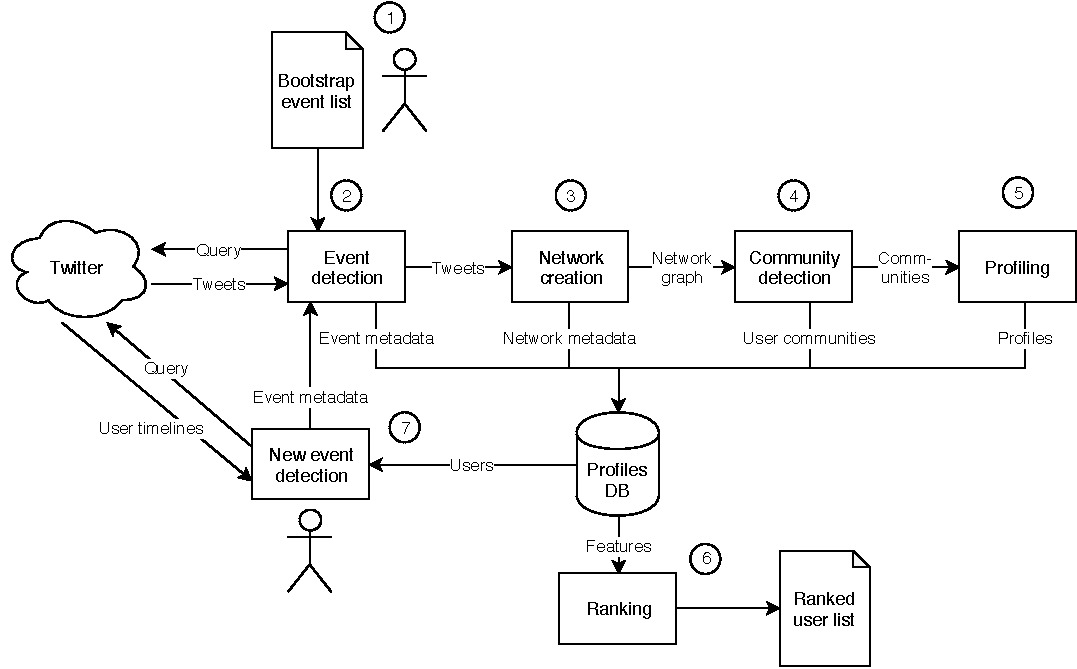
\includegraphics[width=0.7\linewidth]{figures/TwitterFramework}
	\caption{\comment{Schematic diagram of the user discovery framework }{this is a placeholder -- to be redrawn -PM }}
	\label{fig:twitterframework}
\end{figure*}


	
\section{Case study: discovering online activists}

\anote{here we note that functional evaluation was partially carried out in the previous section, while illustrating the pipeline. 
	What we add here: 

\begin{itemize}
  \item comparing users found with influencers on the same case study dataset
  \item comparing different approaches to community detection and user ranking
\end{itemize}

performance: discuss limitations of using the garden hose for content harvesting  (here or in next section??)\\


do we need more than one case study?  My take is that one is good enough for a conference paper --- to be extended later

}
	
	
\section{Discussion and ongoing work}

\anote{
	we say that events are manually identified. Sketch the events bootstrapping idea.
}

 \bibliographystyle{splncs04}
 \bibliography{icwe19}

\end{document}
